\section{Introduction}

L'objectif de ce projet est de réaliser un jeu vidéo massivement multijoueur jouable directement depuis un navigateur web. Ce jeu propose deux modes de jeu bien distincts, offrant aux joueurs des expériences complémentaires :

\begin{itemize}
    \item \textit{Mode "Péon"} : le joueur incarne un personnage individuel et s’occupe d’actions élémentaires comme la collecte de ressources, la construction de bâtiments, ou d'autres tâches concrètes. Ces actions sont réalisées à travers des mini-jeux simples et interactifs.
    \item \textit{Mode "Seigneur"} : le joueur ne contrôle pas directement un personnage, mais adopte une vue stratégique à l’échelle d’un royaume. Il donne des ordres aux péons en fonction des priorités et des besoins du territoire qu’il gouverne.
\end{itemize}

L’univers de jeu est composé de plusieurs royaumes, chacun dirigé par un seigneur différent. Ces royaumes sont en concurrence pour devenir la puissance dominante. Ce système s'inspire librement de la célèbre "Pixel War", un événement sur la plateforme Reddit (r/Place), où des milliers d'utilisateurs ont collaboré ou se sont affrontés pour s’approprier des espaces d’un immense canevas numérique. Bien que purement esthétique, cet événement a généré de véritables dynamiques sociales, entre alliances communautaires et rivalités de territoires. Notre ambition est de transposer ces dynamiques sociales dans un jeu structuré et compétitif, en donnant du sens aux interactions et aux conflits entre joueurs.



\begin{figure}[!h]
   \centering
    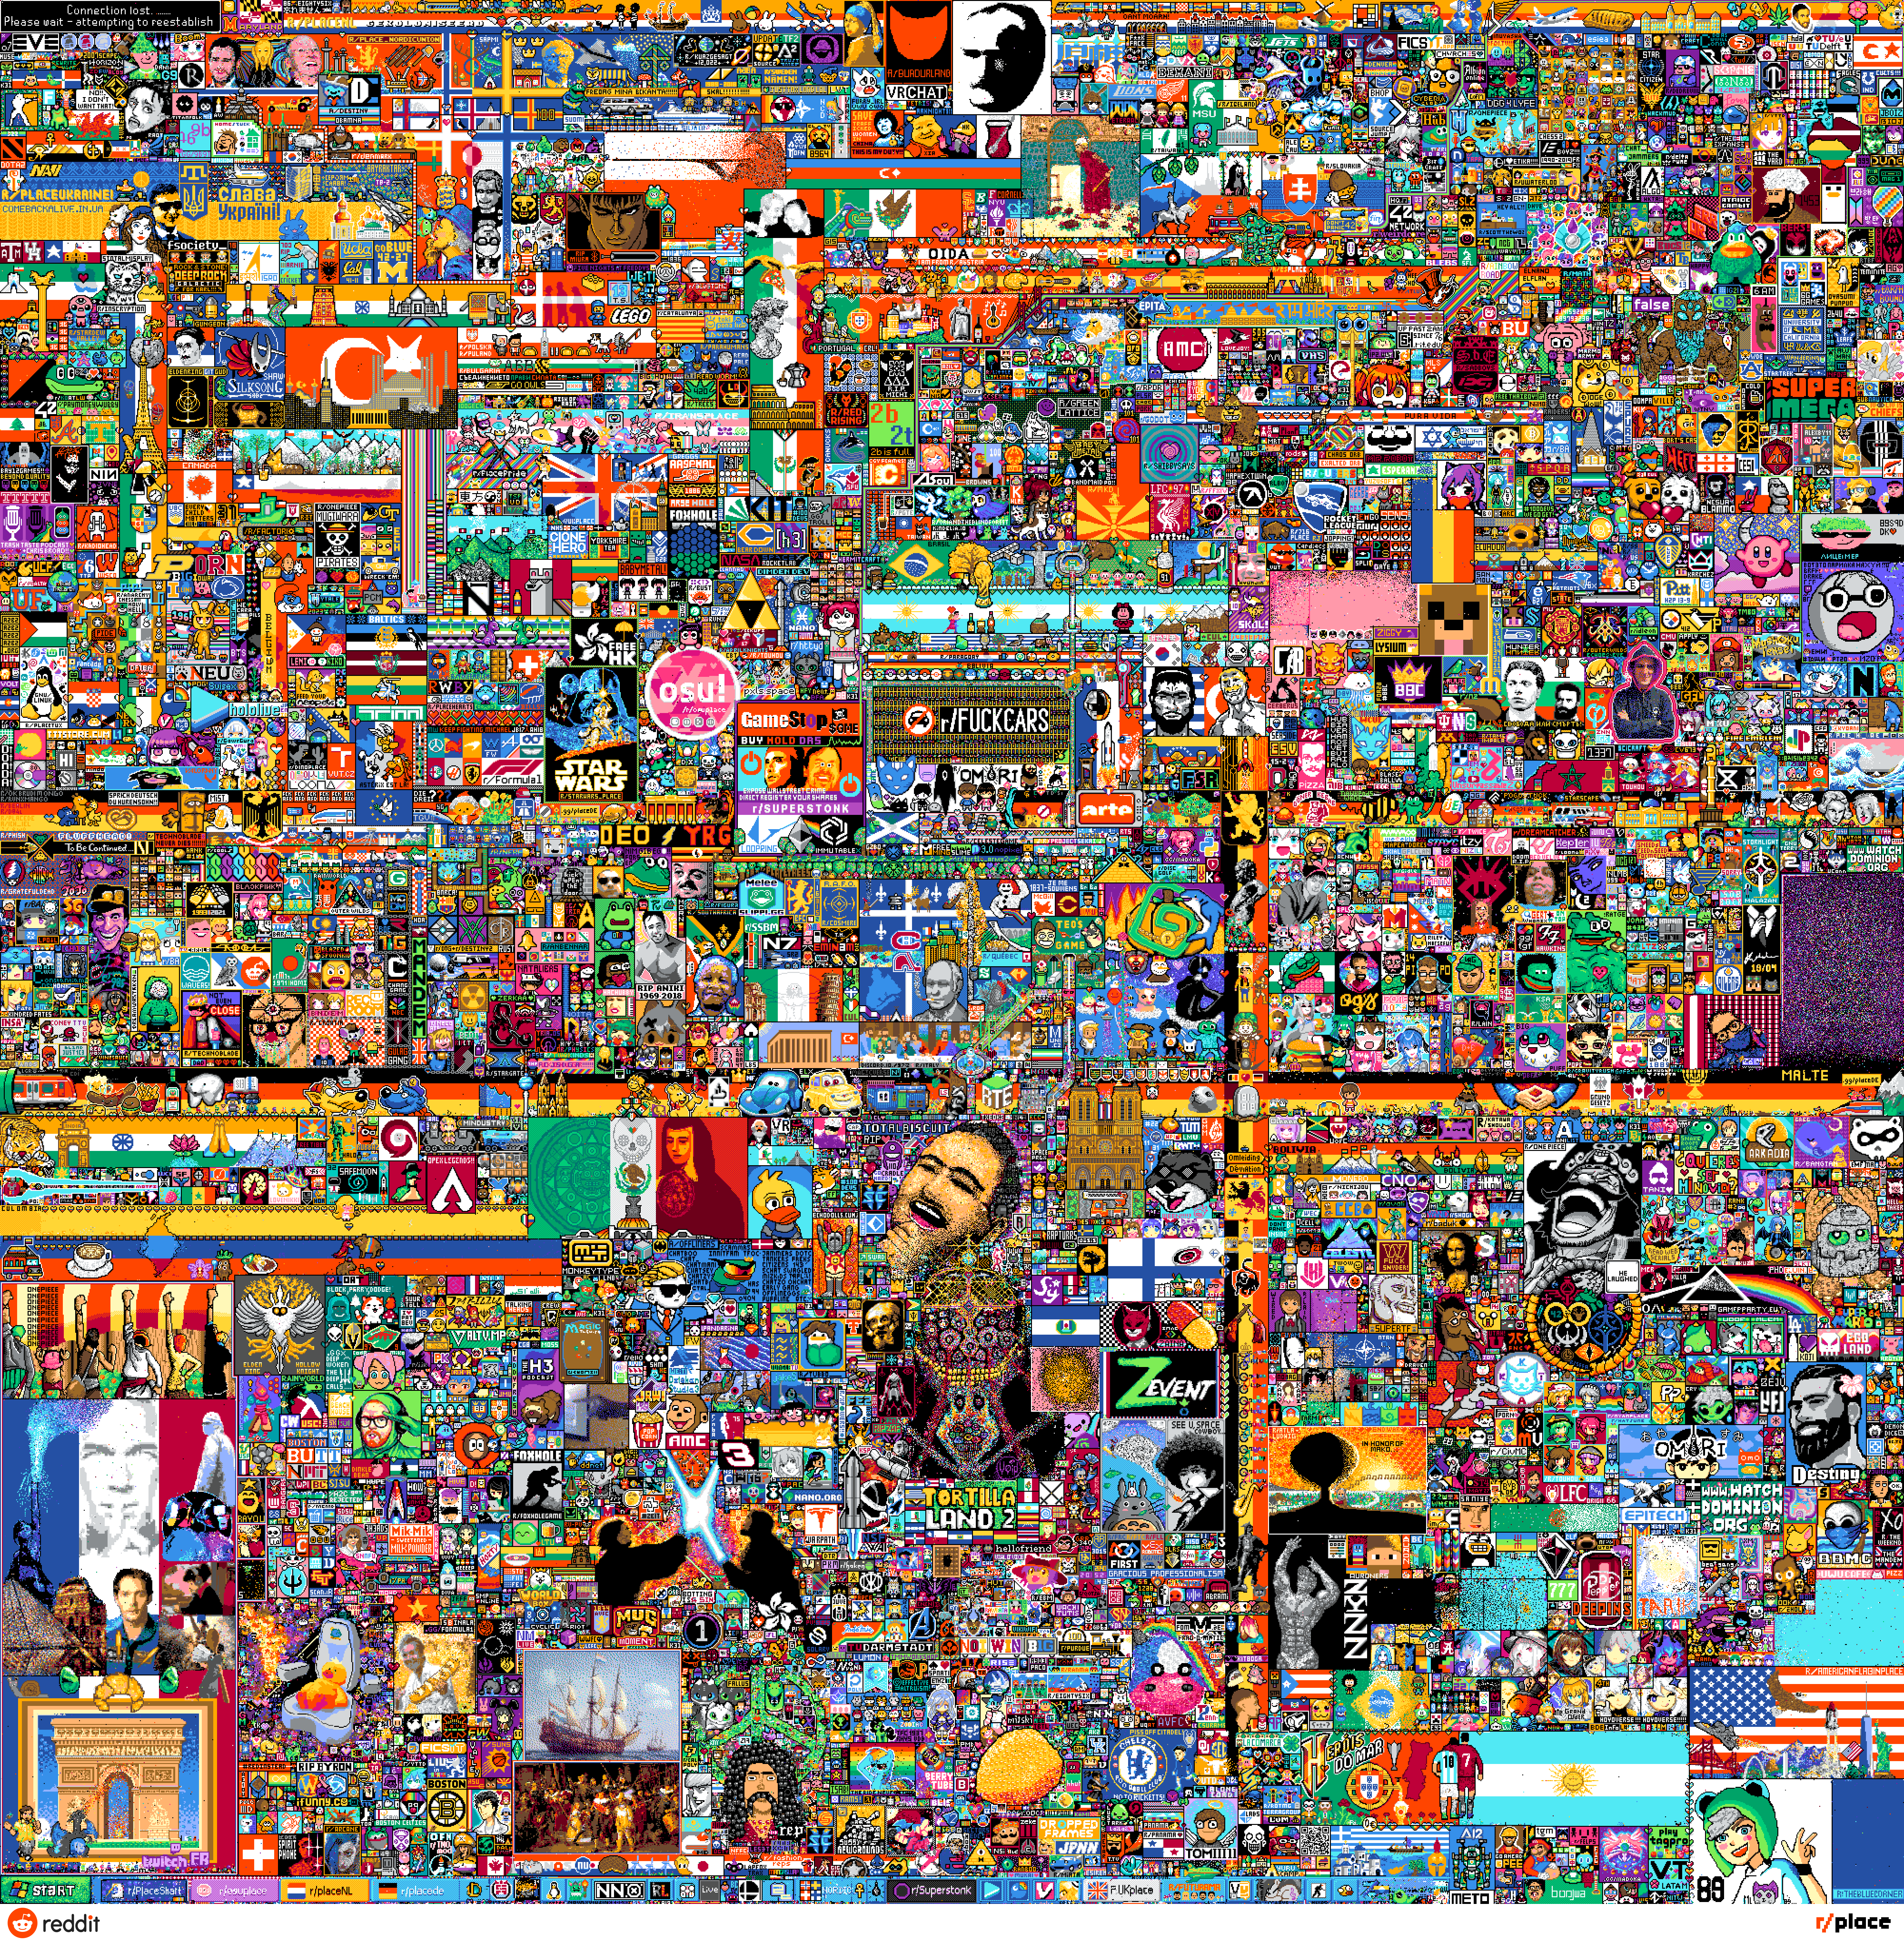
\includegraphics[width=0.5\linewidth]{images/pixelwar.png}
    \caption{Image finale de r/Place}
    \label{fig:pixelwar}
\end{figure}

\paragraph{Étapes et collaboration}
Ce projet, bien que complet en soi, est réalisé en collaboration avec un autre groupe de TER ayant développé un backend scalable destiné à supporter des applications en ligne à fort trafic. Cette coopération nous permet de nous concentrer sur le développement du frontend, tout en assurant une infrastructure serveur solide et adaptée à un jeu massivement multijoueur.

\paragraph{Défis identifiés}
Avant même de commencer le développement, nous avons identifié plusieurs défis techniques et conceptuels majeurs :
\begin{itemize}
    \item Générer une carte procédurale intégrant différentes ressources.
    \item Choisir une technologie adaptée au développement web interactif (WebGL, WebSockets, etc.).
    \item Concevoir un moteur de jeu simple et modulaire.
    \item Développer une interface utilisateur intuitive et réactive.
    \item Créer des mini-jeux simples mais engageants pour les actions de type Péon.
    \item Équilibrer les deux modes de jeu (Péon / Seigneur) pour garantir une jouabilité équitable et cohérente.
    \item Assurer une communication fluide et sécurisée entre frontend et backend.
    \item Créer ou intégrer des assets graphiques adaptés à l’univers du jeu.
\end{itemize}

\paragraph{Portée du projet (MVP)}
Ce projet est ambitieux, et il serait irréaliste de livrer une version complète, stable et publiable dans le temps imparti. C’est pourquoi notre objectif est de développer un \textit{prototype fonctionnel} (MVP – Minimum Viable Product). Ce MVP se concentrera sur l’essentiel : la mise en œuvre des deux modes de jeu, l’interaction avec une carte interactive, et la connexion avec le backend pour la gestion en temps réel des actions des joueurs. Il servira de base pour valider les choix techniques, les mécaniques de gameplay, et les dynamiques collectives que nous souhaitons créer. Ce projet sera continué a la suite de ce rendu dans le but de réelement le lancer en ligne.

\paragraph{Problématique}
\textit{Comment concevoir un prototype fonctionnel de jeu massivement multijoueur sur navigateur qui permette de valider les dynamiques de coopération et de stratégie entre joueurs, tout en intégrant de manière cohérente et interactive deux modes de jeu complémentaires (Péon et Seigneur) ?}
